\documentclass[UTF8, 12pt, a4paper, oneside]{ctexart}
\usepackage{listing}

\usepackage{amsmath}
\usepackage{amsfonts}
\usepackage{geometry}
\usepackage{ulem}
\usepackage[most]{tcolorbox}
\usepackage[hidelinks]{hyperref}
\usepackage{color}
\usepackage{xcolor}
\usepackage{framed}
\usepackage{mdframed}
\usepackage{mathtools,amssymb}
\usepackage{bm}
\usepackage{enumitem}

\definecolor{backcolour}{rgb}{0.18,0.18,0.18}
\definecolor{codegray}{rgb}{0.93,0.93,0.93}
\definecolor{codegreen}{rgb}{0.34,0.76,0.34}
\definecolor{codeblue}{rgb}{0.27,0.35,0.69}
\definecolor{codepurple}{rgb}{0.69,0.25,0.82}
\definecolor{codeorange}{rgb}{0.8,0.6,0.2}
\definecolor{codered}{rgb}{0.8,0.25,0.33}


\lstset{
    backgroundcolor     =   \color{codegray},
    basicstyle          =   \sffamily,          % 基本代码风格
    keywordstyle        =   \bfseries,          % 关键字风格
    commentstyle        =   \rmfamily\itshape,  % 注释的风格,斜体
    stringstyle         =   \ttfamily,  % 字符串风格
    flexiblecolumns,                % 别问为什么,加上这个
    numbers             =   left,   % 行号的位置在左边
    showspaces          =   false,  % 是否显示空格,显示了有点乱,所以不现实了
    numberstyle         =   \zihao{-5}\ttfamily,    % 行号的样式,小五号,tt等宽字体
    showstringspaces    =   false,
    captionpos          =   t,      % 这段代码的名字所呈现的位置,t指的是top上面
    aboveskip           =   1em,
    belowskip           =   1em,
    frame               =   lrtb,   % 显示边框
}

\lstdefinestyle{C++}{
    language        =   C++, % 语言选Python
    basicstyle      =   \zihao{-5}\ttfamily,
    numberstyle     =   \zihao{-5}\ttfamily,
    keywordstyle    =   \color{codepurple},
    keywordstyle    =   [2] \color{codegray},
    stringstyle     =   \color{magenta},
    commentstyle    =   \color{codegreen}\ttfamily,
    breaklines      =   true,   % 自动换行,建议不要写太长的行
    columns         =   fixed,  % 如果不加这一句,字间距就不固定,很丑,必须加
    basewidth       =   0.5em,
}

\lstdefinestyle{C}{
    language        =   C, % 语言选Python
    basicstyle      =   \zihao{-5}\ttfamily,
    numberstyle     =   \zihao{-5}\ttfamily,
    keywordstyle    =   \color{codepurple},
    keywordstyle    =   [2] \color{codegray},
    stringstyle     =   \color{magenta},
    commentstyle    =   \color{codegreen}\ttfamily,
    breaklines      =   true,   % 自动换行,建议不要写太长的行
    columns         =   fixed,  % 如果不加这一句,字间距就不固定,很丑,必须加
    basewidth       =   0.5em,
}

\newlist{choices}{enumerate}{2}
\setlist[choices,1]{
  label = \Alph*.,       % 设置标签格式为大写字母后跟括号,例如 A)、B) 等
  leftmargin = *,        % 设置左边距,使其与上层列表对齐
  align = left,          % 设置标签对齐方式为左对齐
  labelwidth = 1.5em,    % 设置标签宽度
  itemsep = 0.5em        % 设置列表项之间的距离
}

\newmdenv[
  leftmargin=0cm,
  rightmargin=0cm,
  skipabove=1em,
  skipbelow=1em,
  backgroundcolor=gray!20,
  linewidth=0pt
]{mquote}

\title{\texttt{\bf  数据结构 第二次作业}}
\author{学号:2022212408 姓名:胡宇杭}
\date{\today}

\begin{document}
\maketitle

\section{实验目的}
    \begin{enumerate}
        \item 理解 \textbf{\textit{C}} 语言程序的机器级表示;
        \item 初步掌握 \textbf{\textit{GDB}} 调试器的用法;
        \item 阅读 \textbf{\textit{C}} 编译器生成的 \textbf{x86-64} 机器代码,理解不同控制结构生成的基本指令模式、过程的实现;
    \end{enumerate}
\section{双端口存储器实验}
    \subsection{实验目的及任务}
        \begin{itemize}
            \item 实验目的:
            \begin{enumerate}
                \item 了解双端口静态随机存储器 \textit{IDT7132} 的工作特性及使用方法
                \item 了解半导体存储器存储和读取数据的方式
                \item 了解双端口存储器并行读写的方式
                \item 熟悉 \textit{TEC-}8模型计算机存储器部分的数据通路
            \end{enumerate}
            \item 实验任务:
            \begin{enumerate}
                \item 向双端口 \textit{RAM} 的某个地址写入数据(左端口)
                \begin{itemize}
                    \item 向连续的地址写入
                    \item 向非连续的地址写入
                \end{itemize}
                \item 从双端口 \textit{RAM} 的某个地址中读出数据(左、右端口)
                \begin{itemize}
                    \item 从连续的地址读出
                    \item 从非连续的地址读出
                    \item 通过左右端口从同一个地址同时读出
                \end{itemize}
            \end{enumerate}
        \end{itemize}
    
    \subsection{实验电路分析}
        \begin{figure}[htbp]
            \centering
            \includegraphics*[width=12cm]{2_cu.png}
        \end{figure}

        \par 一次完整的运算步骤的电路分析如下:
        \begin{enumerate}
            \item 通过数据开关 \textit{SD}7-\textit{SD}0 将两位 $16$ 进制数输入到 \textit{SWD} 中,当 $SBUS = 1$ 时,数据被送入 \textit{DBUS} 总线上
            \item 令 $LAR = 1$,此时地址寄存器可以写入
            \item \textit{QD},在 $T3$ 时钟上升沿 \textit{DBUS} 上的数据被送入地址寄存器 \textit{AR} 中
            \item 此时 \textit{AR} 中的数据被送至 A7L-A0L 端口,选中对应的内存地址,令 $LAR=0$,关闭地址寄存器写入,令 $MEMW=1$,开启双端口 RAM 的写入功能
            \item \textit{QD},在 $T2$ 时钟上升沿 \textit{DBUS} 上的数据被送入双端口 \textit{RAM} 中由 \textit{AR} 寄存器指定的地址中
            \item 令 $MEMW=0, SBUS=0, MBUS=1$,此时由 $AR$ 选中的内存地址中的数据被送到 \textit{DBUS} 上
        \end{enumerate}

        \subsection{思考题解答}
        \begin{problem}
            如果 \textit{LAR} 为1,45H 是否可以正确写入 23H 单元?
        \end{problem}
        \begin{solution}
            可以正常写入,因为控制内存写入的是 $T2$,比控制 \textit{AR} 写入的 $T3$ 早,所以可以正确写入,但之后 \textit{AR} 被写入 45H,需要重新将 23H 写入 \textit{AR} 才能正确显示
        \end{solution}
        \begin{problem}
            如果 \textit{MEMW}为 1 会发生什么事情?
        \end{problem}
        \begin{solution}
            \textit{MEMW} 为 1 会导致 写入地址时 \textit{RAM} 原来地址位置的数据被覆盖为地址数据
        \end{solution}
        \begin{problem}
            如果 \textit{SBUS} 为 1 会发生什么事情?
        \end{problem}
        \begin{solution}
            不能正常读出,同时控制数据开关,只有原来 \textit{MBUS} 该亮的地方才会亮
        \end{solution}
    
    \subsection{实验过程及结果}
    \begin{table}[htbp]
        \centering
        \scalebox{0.5}{
        \begin{tabular}{|c|>{\centering\arraybackslash}p{4cm}|c|>{\centering\arraybackslash}p{6cm}|>{\centering\arraybackslash}p{3cm}|c|}
            \hline
            \multicolumn{6}{|c|}{\textbf{向10H、20H、21H、22H地址单元写入数据过程}} \\ \hline
            \textbf{序号} & \textbf{操作} & \textbf{数据开关} & \textbf{操作目的} & \textbf{实验现象} & \textbf{备注} \\ \hline
            \textbf{1} & CLR & & 复位 & & \\ \hline
            \textbf{2} & DP=1 & & 设置操作模式 & & \\ \hline
            \textbf{3} & SBUS=1, LAR=1, QD & 10H & 设置第一个写入地址10H,打开SBUS将10H送入数据总线DBUS,同时打开AR的写入信号LAR,按一次QD,将10H地址写入AR & AR=10H & \\ \hline
            \textbf{4} & SBUS=1, MEMW=1, LAR=0, QD & 55H & 设置第一个写入数据45H,打开SBUS将55H送入数据总线DBUS,打开RAM的写入信号MEMW,关闭 AR 的写入信号 LAR,按一次QD, 将 55H 写入 RAM & & \\ \hline
            \textbf{5} & SBUS=1, MEMW=0, LAR=1, QD & 20H & 设置第二个写入地址20H & AR=20H & \\ \hline
            \textbf{6} & SBUS=1, MEMW=1, LAR=0, ARINC=1, QD & AAH & 将 AAH 写入内存地址 20H,同时 AR 自增 & AR=21H & \\ \hline
            \textbf{6} & SBUS=1, MEMW=1, LAR=0, ARINC=1, QD & 10H & 将 10H 写入内存地址 21H,同时 AR 自增 & AR=22H & \\ \hline
            \textbf{7} & SBUS=1, MEMW=1, LAR=0, ARINC=1, QD & 20H & 将 20H 写入内存地址 22H,同时 AR 自增 & AR=23H & \\ \hline
        \end{tabular}
        } 
    \end{table}

    \begin{table}[htbp]
        \centering
        \scalebox{0.5}{
        \begin{tabular}{|c|>{\centering\arraybackslash}p{4cm}|c|>{\centering\arraybackslash}p{6cm}|>{\centering\arraybackslash}p{3cm}|c|}
            \hline
            \multicolumn{6}{|c|}{\textbf{通过左右端口并发从10H、20H、21H、22H地址单元读出数据过程}} \\ \hline
            \textbf{序号} & \textbf{操作} & \textbf{数据开关} & \textbf{操作目的} & \textbf{实验现象} & \textbf{备注} \\ \hline
            \textbf{1} & SBUS=1, MEMW=0, LAR=1, LPC=1, QD & 10H & 将地址10H写入 PC 和 AR & PC=AR=20H IR=INS=55H & \\ \hline
            \textbf{2} & SBUS=0, LAR=0, LPC=0, MBUS=1 & & 左侧读取数据送到 DBUS 上 & D7-D0=55H & \\ \hline
            \textbf{3} & SBUS=1, MEMW=0, LAR=1, LPC=1, QD & 20H & 将地址20H写入 PC 和 AR & PC=AR=20H IR=INS=AAH & \\ \hline
            \textbf{4} & SBUS=0, LAR=0, LPC=0, MBUS=1 & & 读出 20H 的数据 & D7-D0=AAH & \\ \hline
            \textbf{5} & SBUS=0, ARINC=1, LAR=0, LPC=0, PCINC=1, MBUS=1, QD & & AR、PC自增,读出 21H 的数据 & PC=AR=21H D7-D0=10H IR=INS=10H & \\ \hline
            \textbf{6} & SBUS=0, ARINC=1, LAR=0, LPC=0, PCINC=1, MBUS=1, QD & & AR、PC自增,读出 22H 的数据 & PC=AR=22H D7-D0=20H IR=INS=20H & \\ \hline
        \end{tabular}
        } 
    \end{table}

    \subsection{实验收获及体会}
        \par 知道了计算机如何向存储器中写入和读出数据,如何连续的存储和读取数据

    
\section{实验内容}
    \subsection{问题描述:}
        \par 哈夫曼编码是一种基于最优二叉树的无损编码方案。需要根据字符集和频度的实际统计构建哈夫曼树,然后进行编码和译码。
    \subsection{要求:}
        \begin{itemize}
            \item \textbf{初始化:} 从终端读入字符集大小 \textbf{n},以及 \textbf{n} 个字符和 \textbf{n} 个权值,建立哈夫曼树,并将它存于文件 \textbf{hfmTree} 中;
            \item \textbf{编码:} 利用已经建好的哈夫曼树,对文件 \textbf{ToBeTran} 中的报文进行编码,然后将结果存入文件 \textbf{CodeFile} 中(为简化处理,可以在 \textbf{CodeFile} 中用一个字节来存储码字中的一个 \textbf{0/1} 比特位);
            \item \textbf{译码:} 利用已建好的哈夫曼树,对 \textbf{CodeFile} 中的代码进行译码,结果存入 \textbf{TextFile} 中。
        \end{itemize}
    \subsection{附加要求:}
        \par 对一个 \textbf{512*512} 的 \textbf{lena.bmp} 灰度图片进行哈夫曼编码。\textbf{BMP} 文件由:\textbf{BMP} 文件头 $+$ 像素数据组成,灰度图 \textbf{1} 个像素占用 \textbf{1} 个字节。\textbf{lena.bmp} 文件大小是 \textbf{263222} 字节,包括 \textbf{1078} 字节的头部 $+$ \textbf{512*512} 个像素值。\textbf{lena.bmp} 文件见实验作业附件。
        
\section{实验步骤}
    \textbf{操作步骤+运行截图}
    \subsection{实验内容一}
        \subsubsection{代码解释}
            \subsubsection*{基础功能}
                \begin{enumerate}
                    \item 定义学生结构体,数据项包含学号、姓名、年龄。
                        \begin{figure*}[htbp]
                            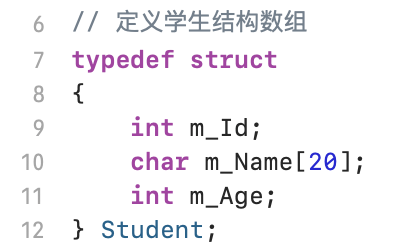
\includegraphics[width = 7cm]{work1_s1.png}
                        \end{figure*}
                    \item 将学生结构体封装进线性表,便于后续文件读写操作。
                        \begin{figure*}[htbp]
                            \includegraphics*[width = 15cm]{work1_s2.png}
                        \end{figure*}
                    \newpage
                    \item \textbf{\textit{init()}} 函数用于从 \textbf{\textit{input.dat}} 中读取数据初始化线性表,如果没有任何数据,则会将表长初始化为 \textbf{\textit{0}},否则将会读入历史数据。
                        \begin{figure*}[htbp]
                            \includegraphics*[width = 14cm]{work1_s3.png}
                        \end{figure*}
                \end{enumerate}
            \subsubsection*{功能项 1}
                \par 依次输入五名学生的信息,由于学号递增,只需输入第一位学生的学号。
                \par \textbf{\textit{index}} 可以表示表长,同时也表示指向表尾后一位的指针,这就代表我们可以通过 \textbf{\textit{index}} 向线性表中添加元素。
                \par 因此每次只要将学生添加到数组下标为 \textbf{\textit{index}} 的位置,并在一次迭代结束时令 \textbf{\textit{index ++ }},使其指向下一个位置。
                \begin{figure*}[htbp]
                    \includegraphics*[width = 17cm]{work1_s4.png}
                \end{figure*}
            \newpage
            \subsubsection*{功能项 2}
                \par 以二进制方式写入文件,如果文件无法打开,则抛出异常,否则将表长和学生结构体数组存入 \textbf{\textit{input.dat}} 中。
                \begin{figure*}[htbp]
                    \includegraphics*[width = 12cm]{work1_s5.png}
                \end{figure*}
            \subsubsection*{功能项 3}
                \par 由于我们需要将一个文件里的数据逆序写入到另一个文件中,所以需要创建一个临时的线性表接受数据,再将其逆序写入新的文件中。
                \par 在程序中,首先创建了临时变量 \textbf{\textit{temp}},并将 \textbf{\textit{input.dat}} 的数据读入 \textbf{\textit{temp}} 中,同时由于读入学生结构体数组时需要用到线性表的表长,因此先读入表长,这也是存储时先存储表长的原因。
                \par 在写入时,我们从数组下标为 \textbf{\textit{index - 1}} 处开始写入,以此实现逆序输出的要求。
                \begin{figure*}[htbp]
                    \includegraphics*[width = 11cm]{work1_s6.png}
                \end{figure*}
            \subsubsection*{附加要求}
                \par 具体实现见运行截图中的说明。
        \subsubsection{运行截图}
            \begin{enumerate}
                \item 在 \textbf{\textit{func1()}} 循环中设置条件断点。
                \begin{figure*}[htbp]
                    \centering
                    \includegraphics*[width = 10cm]{work1_s7.png}
                \end{figure*}
                \item 运行程序,可以看到,程序在执行到处理第 $5$ 位学生信息时中断。
                \begin{figure*}[htbp]
                    \centering
                    \includegraphics*[width = 10cm]{work1_s8.png}
                \end{figure*}
                \item 继续运行,程序结束
                \newpage
                \item 第二次运行程序,我们可以在监视栏看到上一次运行的数据被成功保存并读入进来。
                \begin{figure*}[htbp]
                    \centering
                    \includegraphics*[width = 10cm]{work1_s9.png}
                \end{figure*}
                \item 继续运行,发现由于 \textbf{\textit{index}} 的存在,使得程序可以正确地从上一次截止位置继续添加学生信息。
                \begin{figure*}[htbp]
                    \centering
                    \includegraphics*[width = 10cm]{work1_s10.png}
                \end{figure*}
                \newpage
                \item 第三次运行程序,我们修改 \textbf{\textit{init()}} 函数的参数,从 \textbf{\textit{output.dat}} 中读入数据,并输出。
                \begin{figure*}[htbp]
                    \centering
                    \includegraphics*[width = 10cm]{work1_s11.png}
                \end{figure*}
                \item 可以看到,输出的内容是逆序的,说明我们在上两次程序中成功将数据逆序存储到了 \textbf{\textit{output.dat}} 中。
                \begin{figure*}[htbp]
                    \centering
                    \includegraphics*[width = 10cm]{work1_s12.png}
                \end{figure*}
            \end{enumerate}
    \subsection{实验内容二}
        \subsubsection{实验步骤}
            \subsubsection*{代码实现}
                \par 此处 \textbf{\textit{copyij}} 和 \textbf{\textit{copyji}} 函数与提供的一致,\textbf{\textit{N}}为 \textbf{\textit{2048}}, 故此处只给出主函数的实现。
                \begin{figure*}[htbp]
                    \includegraphics*[width = 15cm]{work2_s1.png}
                \end{figure*}
            \subsubsection*{两个函数的运行时间比较及原因分析}
                \begin{figure*}[htbp]
                    \centering
                    \includegraphics*[width = 15cm]{work2_s2.png}
                \end{figure*}
                \par 从图中不难看出,\textbf{\textit{copyij}} 的执行效率远高于 \textbf{\textit{copyji}},通过查阅相关资料(CSDN,CSAPP等),现给出如下解释:
                \par \textbf{\textit{copyij}} 和 \textbf{\textit{copyji}} 的主要差异在于其遍历数组的顺序,\textbf{\textit{copyij}} 是按行遍历,而 \textbf{\textit{copyji}} 是按列遍历。
                \par 我们知道,在 \textbf{\textit{C}} 和 \textbf{\textit{C++}} 中,二维数组采用行优先存储,并且计算机在访问一块内存空间时,会有以下性质:
                \begin{itemize}
                    \item 空间局部性:当一个内存位置被访问时,通常其附近的内存位置也会在不久后被访问。这为缓存行提供了理论基础。
                    \item 缓存行:处理器缓存不是以单个字节或字为单位来缓存的,而是以 ``缓存行'' 为单位。缓存行通常包含多个连续的内存位置。当我们访问一个特定的内存位置时,整个缓存行都会被加载到缓存中。因此,紧接着访问该缓存行中的其他位置将非常快速。
                    \item 预取:现代处理器通常有预取单元,它们可以预测程序下一步可能需要哪些数据,并在它们实际需要之前将这些数据加载到缓存中。
                \end{itemize}
                \par 有上述几点性质,我们再来看这两个函数,在 \textbf{\textit{copyij}} 函数中,按行顺序遍历会使得更多的访问命中缓存,因为它们都在同一个或相邻的缓存行中,并且连续内存访问模式更容易被预取单元预测,从而提高效率。相比之下,\textbf{\textit{copyji}} 则没有这些优点。
            \subsubsection*{时间复杂度分析}
                \par 从运行结果上来看,两个函数的作用都是将一个二维数组的元素复制到另一个二维数组中,外层都循环 \textbf{\textit{N}} 次,内层也都循环 \textbf{\textit{N}} 次,因此,两个函数的时间复杂度均为 $\theta(N^2)$。
            \subsubsection*{附加要求}
                \begin{figure*}[htbp]
                    \centering
                    \includegraphics*[width = 7cm]{work2_s3.png}
                    \includegraphics*[width = 7cm]{work2_s4.png}
                    \caption{左:关闭O2优化 右:开启O2优化}
                \end{figure*}
                \par 比较关闭 \textbf{\textit{O2}} 优化和开启 \textbf{\textit{O2}} 优化时程序执行所用时间,不难得出:
                \begin{itemize}
                    \item 开启 \textbf{\textit{O2}} 优化时 \textbf{\textit{copyij}} 的执行时间更短。
                    \item 开启 \textbf{\textit{O2}} 优化时 \textbf{\textit{copyji}} 的执行时间反而更长。
                \end{itemize}
        \newpage
        \subsubsection{运行截图}
            \begin{itemize}
                \item 通过命令行关闭和开启 \textbf{\textit{O2}} 优化。
                \begin{figure*}[htbp]
                    \centering
                    \includegraphics*[width = 13cm]{work2_s5.png}
                \end{figure*}
                \item 创建出的两个可执行文件。
                \begin{figure*}[htbp]
                    \centering
                    \includegraphics*[width = 13cm]{work2_s6.png}
                \end{figure*}
                \item 程序在 \textbf{\textit{Xcode}} 的运行截图。
                \begin{figure*}[htbp]
                    \centering
                    \includegraphics*[width = 14cm]{work2_s7.png}
                \end{figure*}
                \newpage
                \item 程序在终端的运行截图
                \begin{figure*}[htbp]
                    \centering
                    \includegraphics*[width = 7cm]{work2_s3.png}
                    \includegraphics*[width = 7cm]{work2_s4.png}
                    \caption{左:关闭O2优化 右:开启O2优化}
                \end{figure*}
            \end{itemize}
         



\end{document}